\chapter{Experiment Design}

This chapter defines how the desired outcomes defined in the Methodology will practically be met. This requires describing the available code and data, how it will integrate with new code developed in this project and what the new code being developed is.

Additionally, this chapter describes existing work and data to the reader.

\subsection{Well Data in iArsenic}

The data used by iArsenic can be found in the CSV in the data/ directory of iArsenic (note that this does not include CSV files in sub-directories of the data/ directory). These files have been selected on the following criteria for aggregating:

\begin{itemize}
    \item two CSV files do not include the same datapoint
    \item the CSV contains standard features required by the iArsenic models
\end{itemize}

Before preprocessing, these files contain 1,144,586 rows (including headers) combined.

The primary preprocessing function provided by iArsenic is name correcting. This is the process of renaming region names such that a region with different names in different datasets, has the same name in an aggregate dataset. These corrections allow the well data and the geodata to be aggregated. Most name differences are caused by differences in phonetic translation or inconsistent capitalisation.

After preprocessing, the iArsenic data source contains 868,679 rows (including headers).

See figure \ref{fig:x avg_datapoints} on page \pageref{fig:x avg_datapoints} for a choropleth of datapoints per District.

\begin{figure}[!htb]
    \centering
    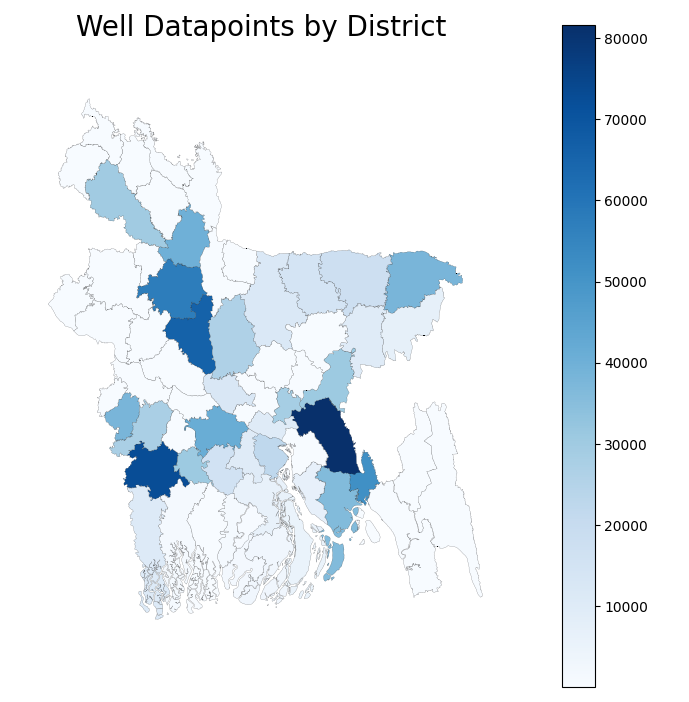
\includegraphics[scale=0.6]{figures/data_distribution_by_district.png} 
    \caption{Distribution of Well Data by District in iArsenic Processed Dataset}
    \label{fig:x avg_datapoints}
\end{figure}

The attributes included in the aggregate data file output by iArsenic are the following:

\begin{itemize}
    \item Division
    \item District
    \item Upazila
    \item Union
    \item Mouza
    \item Depth
    \item Arsenic
\end{itemize}

Excluding Depth and Arsenic, these attributes are all region names with corresponding geographic data. 

See figure \ref{fig:x labelled_divisions} on page \pageref{fig:x labelled_divisions} for a labelled map of Bangladesh divisions.

\begin{center}
    \begin{tabular}{|c c c c|} 
         \hline
         Name & Mean Area $km\textsuperscript{2}$ & Mean Area $\sigma$ & Unique Values \\ [0.5ex] 
         \hline\hline
         Division & 17,482 & 6,928 & 8 \\ 
         \hline
         District & 2,185 & 1,080 & 63 \\
         \hline
         Upazila & 257 & 185 & 445 \\
         \hline
         Union & 27 & 41 & 2,838 \\
         \hline
         Mouza & 2.4 & 8.4 & 9,550 \\ [1ex] 
         \hline
    \end{tabular}
\end{center}

\begin{figure}
    \centering
    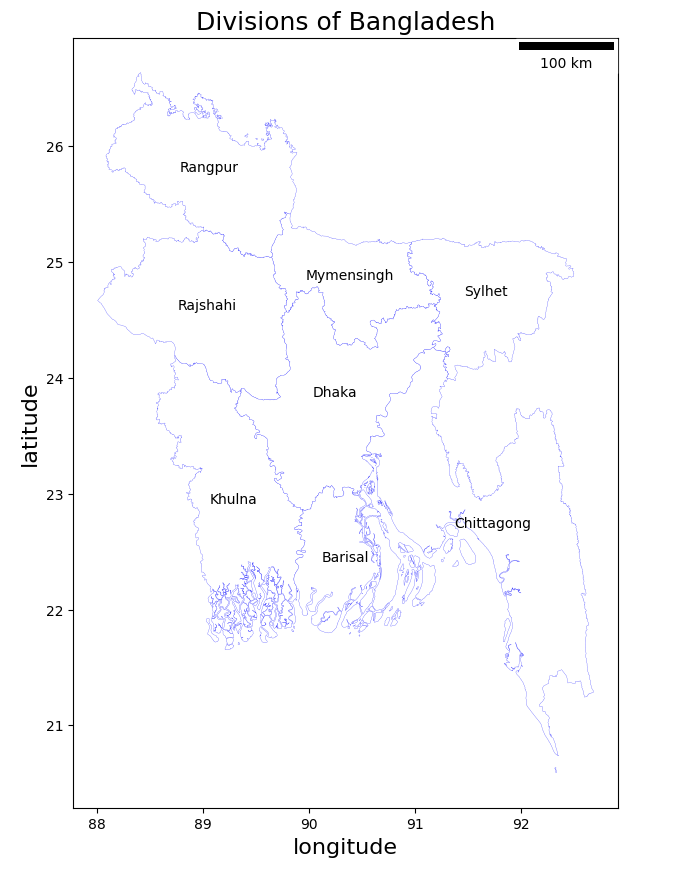
\includegraphics[scale=0.6]{figures/labelled_divisions.png} 
    \caption{The regions of Bangladesh as per the iArsenic dataset}
    \label{fig:x labelled_divisions}
\end{figure}

\textbf{Depth}

The Depth column refers to the depth of a well in meters.

The deepest well in the dataset is 445 meters, the lowest is 0, the is mean 40 meters and the standard deviation is 52 meters. See figure \ref{fig:x avg_depth} on page \pageref{fig:x avg_depth} for a choropleth of mean depth per Upazila.

\begin{figure}[!htb]
    \centering
    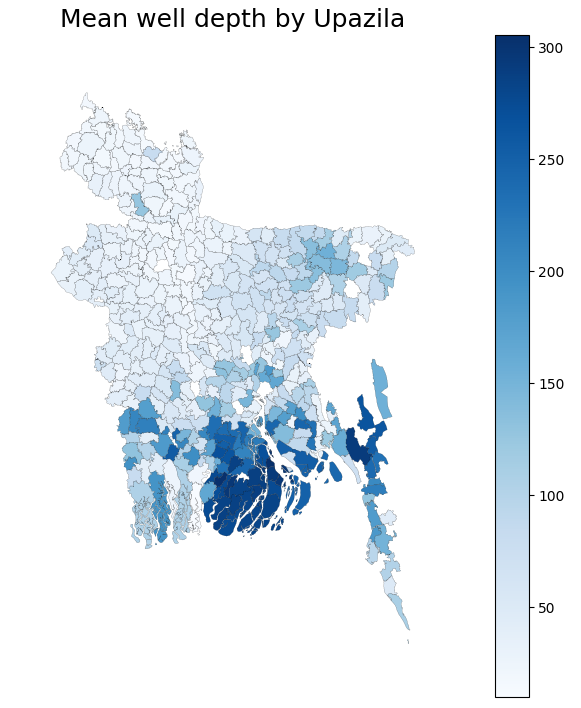
\includegraphics[scale=0.6]{figures/mean_well_depth_by_upa.png} 
    \caption{Average (mean) Well Depth by Upazila}
    \label{fig:x avg_depth}
\end{figure}

\textbf{Arsenic}

The Arsenic column refers to the arsenic concentration in water from a well datapoint in micrograms per litre ($\mu$g/l).

The highest concentration of arsenic in the dataset is 4,000$\mu$g/l (4ng/l), the lowest concentration of arsenic is 0$\mu$g/l, the mean is 41$\mu$g/l and the standard deviation is 74$\mu$g/l. See figure \ref{fig:x avg_as} on page \pageref{fig:x avg_as} for a choropleth of mean depth per Upazila.

\begin{figure}[!htb]
    \centering
    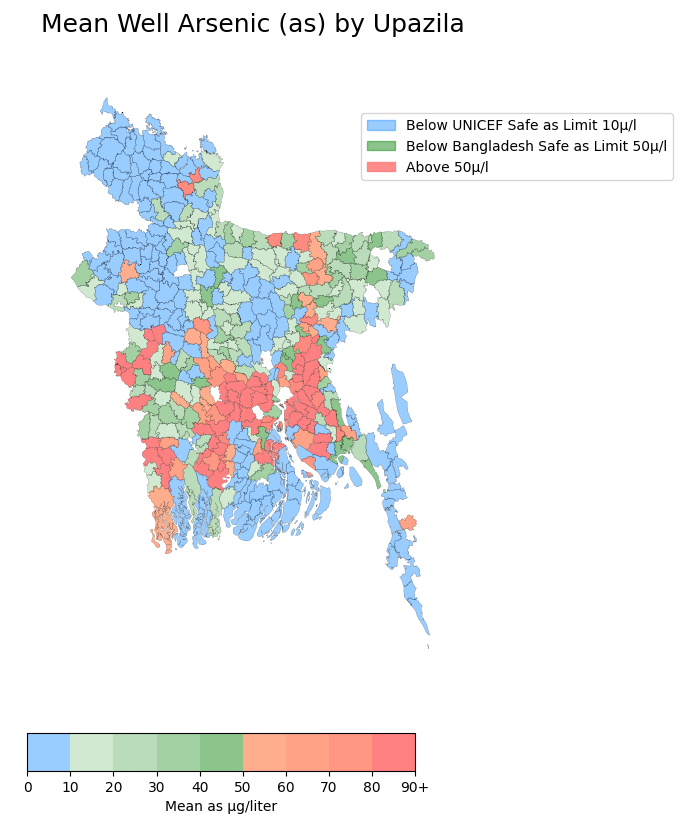
\includegraphics[scale=0.6]{figures/mean_as_by_upazila.png} 
    \caption{Distribution of Average (mean) Arsenic by Upazila in Preprocessed iArsenic Dataset}
    \label{fig:x avg_as}
\end{figure}

\newpage

\textbf{Why use this Dataset?}

While new and existing iArsenic models could be trained on different data, the time and resources required to produce a dataset of this quality and suitability are substantial and outside the scope of this project. 

\subsection{Geodata}

The original source of the geodata is unclear, though similar country based polygon data can be found on the first page of google.

% reference where these instructions are in iArsenic
The geodata has been zipped and added to the project's repository using Git Large File Storage. This is because some of the geodata is omitted from the original iArsenic repository due to it exceeding the GitHub file size limit. Instructions are provided in iArsenic for regenerating this missing data.

\section{iArsenic Integration}

\subsection{Data Preparation}

The iArsenic code repository is downloaded from GitHub via Node Package Manager (npm). This repository includes selected source data and several tools to process this data.

% TODO reference csv-to-json script in appendix
Data is extracted from iArsenic using the csv-to-json.js script. This script aggregates the source files into a single data structure and outputs it as a JSON file. Additionally, it ensures that all regions follow the same naming convention, which is essential because it prevents distinct data points in the same region from appearing to be in two different regions. This enables the data to be matched to its corresponding polygon in the geodata.

% TODO reference the utils/src_to_test_train.py script and the generated files
The JSON file is then converted to a pandas DataFrame in Python, shuffled to ensure there is no ordering bias, and converted into 5 separate CSV files. It is split into 5 to enable k-fold cross-validation on the dataset.

These 5 CSV files are what we use to test and train the models.

\subsection{Generating the iArsenic Models}

iArsenic can generate 3 separate models: model3, model4 and model5.

Originally an iArsenic model was generated on all available data and then made available on the iArsenic webpage. Due to their modular design however, the models can also be imported into NodeJS code.

To evaluate the models using k-folds cross-validation, each of the 3 models was generated 5 times with 4 of the CSVs used for training and 1 for testing, thus implementing k-folds cross-validation. This generated a total of 15 iArsenic models.

\subsection{Interfacing With Generated iArsenic Models}

% TODO reference iarsenic-wrapper.js
% TODO explain that the ia models generate multiple classifications but have been simplified to safe or not safe
Predictions are generated from the generated model using a NodeJs wrapper script. This will be referred to as the iArsenic Model Wrapper

The predictions are saved to a temporary CSV file and the name of this file is logged to the standard output.

The wrapper script requires the following parameters to be passed as system arguments:
\begin{itemize}
  \item a CSV file containing the data points to use to generate predictions
  \item the stain colour of the well the data point is from
  \item the model to generate the prediction from
  \item the k-fold version of the model to generate the prediction from
\end{itemize}

Initially, the wrapper script would produce an estimate from one data point at a time, passed as a system argument. However, this took more time than pracitcal to process when passing the test dataset. Therefore the test dataset is passed as a CSV filepath.

% TODO specify what is the source data, maybe have raw data, source data and kfolds data
% TODO link to section in evaluation
% TODO include a chart showing the performance with different colours for models34&5

\subsection{Imputing Stain Colour}

In the original iArsenic webpage, the stain colour was to be specified by a user entering parameters about a real well, allowing the user to observe and provide the staining colour of the well. The data extracted from iArsenic however did not include staining colour data. 

When working with missing values there are primarily 3 options: 

% TODO reference handson ml scikit learn here
\begin{enumerate}
    \item remove the feature with missing values
    \item delete all rows containing missing data
    \item replace missing data with a fixed value
\end{enumerate}

Because the iArsenic models will not run with the colour omitted, option 1 is not viable. Because none of the rows contain staining data, option 2 is also not viable. Therefore we must fill in the data with a fixed value, either 'Red' or 'Black'.

To determine whether the value should be set to 'Red' or 'Black', the models have been evaluated using each and the value with which the model performs best, 'Red', has been selected. Figure \ref{fig:x ia_model_black_red_accuracy} on page \pageref{fig:x ia_model_black_red_accuracy} shows the accuracy of the iArsenic models with 'Black' or 'Red' used as the imputed well colour.

\begin{figure}[h]
    \centering
    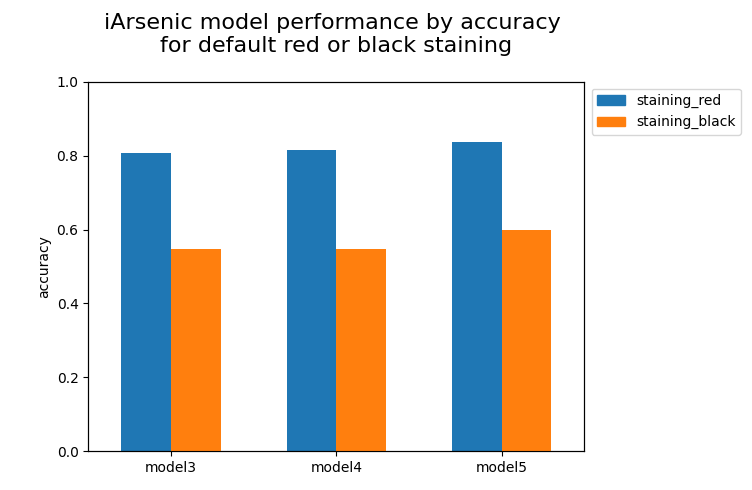
\includegraphics[scale=0.55]{figures/ia_model_black_red_accuracy.png} 
    \caption{iArsenic model performance by accuracy for default red vs black staining}
    \label{fig:x ia_model_black_red_accuracy}
\end{figure}

\newpage

% TODO maybe reference the number of positives and negatives in the original dataset
Considering the accuracy score alone, it would appear that setting the parameter to 'Red' produces the best model performance by approximately 10\%. A higher accuracy score however does not guarantee that one model outperforms another. This could happen because the source data has a much higher positive than negative rate and the model always predicts positive for example. Therefore specificity and sensitivity must also be considered.

Comparing the sensitivity and specificity of the models shows that when the staining is set to 'Black' model3 and model4 always assume the well is safe. The sensitivity, the true positive rate, becomes 0 and the specificity, the true negative rate, becomes 1. Occasionally model5 will classify black staining as polluted but the specificity is effectively 0. While the specificity is lower when the staining is set to 'Red', the sensitivity is much higher for each model, indicating better performance.

\newpage

\begin{figure}[!htb]
    \centering
    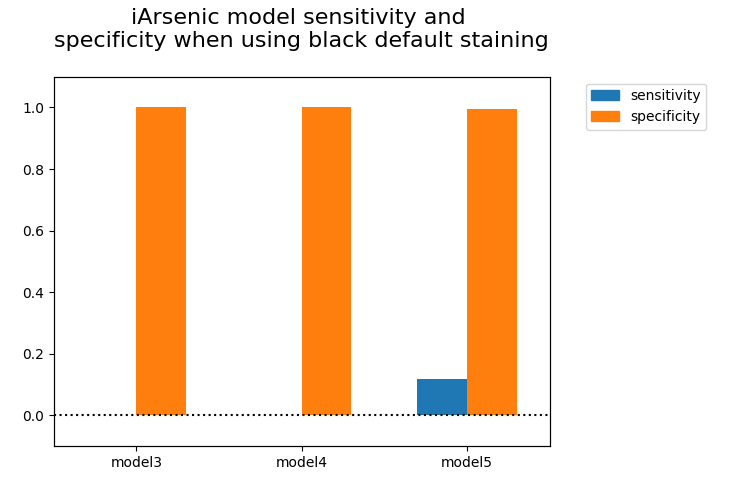
\includegraphics[scale=0.55]{figures/ia_models_sensitivity_vs_specificity_black.png} 
    \label{fig:x ia_svs_black}

    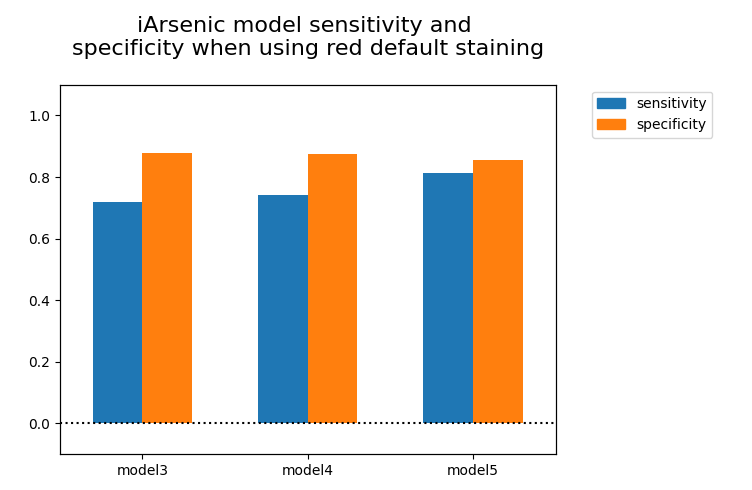
\includegraphics[scale=0.55]{figures/iarsenic_model_sensitivity_vs_specificity_red.png} 
    \caption{Model sensitivity and specificity stain parameter 'Black' (top) vs 'Red' (bottom)}
    \label{fig:x ia_svs_red}
\end{figure}

\newpage

Generating two confusion matrices for model5, one generated from 'Black' passed as a parameter and one from 'Red', reinforces the conclusion that using 'Red' as a parameter produces a better model.

\begin{figure}[!htb]
    \centering
    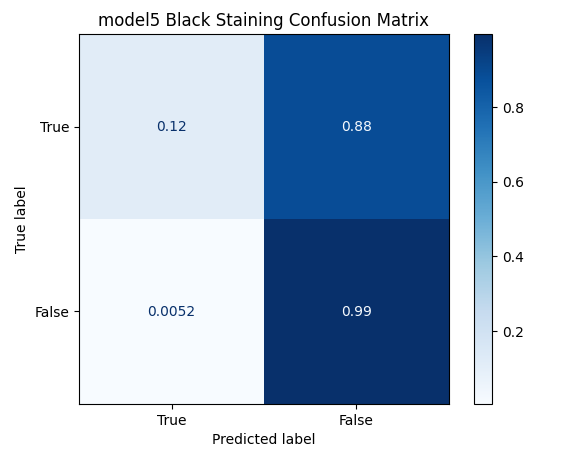
\includegraphics[scale=0.6]{figures/m5_black_cm.png} 
    \label{fig:x Confusion Matrix mode5 Black Staining}
    
    \centering
    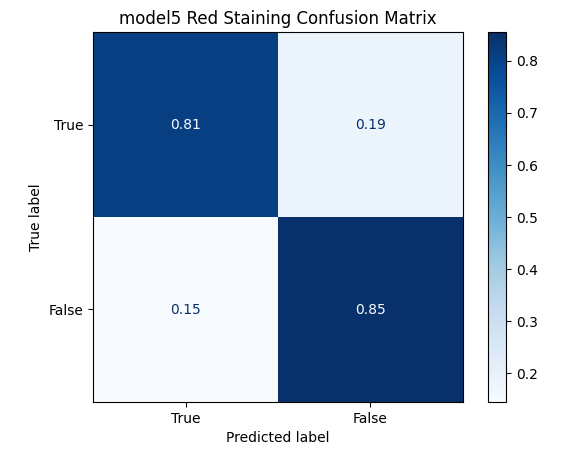
\includegraphics[scale=0.6]{figures/m5_red_cm.png} 
    \caption{Confusion Matrix model5 'Black' (top) vs 'Red' (bottom) Staining}
    \label{fig:x Confusion Matrix mode5 Red Staining}
\end{figure}

\newpage

\textbf{Qualitative Approach to Selecting Staining Parameter}

Observing the evaluation metrics of the iArsenic models and comparing them when producing predictions with either 'Red' or 'Black' as the staining parameter has indicated that the models perform better with 'Red' passed as a parameter. This is however still arguably down to interpretation.

A qualitative comparison of the models, using a value such as Area Under the Curve (AUC) would be preferable. This however is not possible with the iArsenic models as there is no feature to change the classification threshold, which is required to generate a Receiver Operating Curve (ROC) and therefore calculate AUC.

\section{Generating the Machine Learning Models}

The machine learning models are made with scikit-learn in Python. 

Each model is defined in an individual Python script and exported as a Python module.

\section{Creating a Common Model Interface}

The machine learning models will be made in Python. These can be interfaced with directly using Python modules with parameters passed directly into function calls. This is inconsistent with the iArsenic models which are run via the iArsenic wrapper with node, passing parameters using command line arguments.

A Common Module Interface has therefore been specified which standardises how the modules should be interacted with. This interface specifies that each model will have a main function which takes two parameters, the test data source and the k-fold number and rehouseturns predictions as a pandas dataframe. Each model can be run via a Python module that follows this standard.

\subsection{Implementing the Common Model Interface}

% TODO display some kind of figure or diagram of the file structure, possibly a generic and an example
Each model has a directory in the top level models directory. Each model directory contains a model.py file which exports a Python module which can generate predictions based on the Common Module Interface, in addition to any other resources required by the model.

% TODO reference gen_predictions in ia_model_wrap.py
The iArsenic Model Wrapper cannot accept variables passed by Python. Therefore a Python to NodeJS Bridge has been created. The Python to NodeJS Model Bridge works by running the iArsenic Model Wrapper from Python in a subprocess managed by Python.

The Python to NodeJS Bridge can then be imported to the top level main.py script.

\section{Evaluating the Models}

% TODO refer to these terms explained in the literature review, not explained in this e
The predictions returned from the common model interface are used for evaluation. The follow evaluation metrics are generated:
\begin{itemize}
  \item accuracy (\(\frac{true\_positives + true\_negatives}{total\_predictions}\))
  \item sensitivity (\(\frac{true\_positive}{true\_positive + false\_negative}\))
  \item precision (\(\frac{true\_positive}{true\_positive + false\_positive}\))
  \item specificity (\(\frac{true\_negative}{true\_negative + false\_positive}\))
  \item f1 score (\(\frac{precision * sensitivity}{precision + sensitivity}\))
\end{itemize}

\section{Creating a Main Script to Run \& Evaluate Experiments}

The Common Module Interface allows the models imported to the main.py script and run programmatically, without specific code defined for each model. 

This facilitates maintainable code as the complexity of the code increases. The complexity of the main.py script necessitates steps to ensure maintainability are taken. 

Significant complexity has been introduced in making the models run and build concurrently. This is important however as doing this sequentially would take more time than is practical.

While the iArsenic models benefit the most from being run concurrently, as these are single threaded, so running them concurrently allows more of the host machine's CPU power to be utilised by using multiple CPU cores.

The machine learning models however are written using scikitlearn libraries, which are able to use all CPU cores available. 

Further optimizing the models by, for example, running the iArsenic models concurrently and the machine learning models sequentially was not deemed necessary, as building and running all models concurrently took approximately 3.5 days, which is a practical amount of time. This run was achieved on a server computer with Ubuntu 22.01, an 8 x 1.8GHz core CPU and 96GB 1600MHz DDR3 RAM.

\subsection{Main Script Structure}

The purpose of the main.py script is to provide an entrypoint to execute all required steps of the project.

The main script takes the following steps:
\begin{enumerate}
    \item extract the iArsenic \& geodata
    \item generate the k-folds cross-validation data split 
    \item build the iArsenic models
    \item generate predictions from all models
    \item generate an evaluation for each model's predictions
\end{enumerate}

\section{Development of New Models}

%Introduction to the process taken for each model, hypothesizing why a hypothetical model would work then explaining the preprocessing required and implementation.

%- models are developed using typical supervised learning models like RF KNN 

%- regression models are not used as the purpose of the models is to compare with the existing iArsenic models which are classification 

\subsection{model6}

Model6 is an implementation of scikit-learn's random forest classifier with the default configuration.

Because this model cannot process string values, all string values are converted to numerical values, with each new string given an identification number in ascending order.

\subsection{model7}

model7 is also a default implementation of scikit-learn's random forest classifier. This model incorporates computed region attributes computed in model5.

model5 uses feature engineering to calculate the median, lower quartile and upper quartile of the arsenic in a region, for a given depth range.

The hypothesis is that this feature engineering will provide the model with information that correlates with the model prediction target for a given datapoint, improving the models performance.

These values are therefore incorporated into the dataset used for model7. Where the values for a region are missing from the model5 dataset, the values from the region's parent are used.

\subsection{model8}

model8 uses a feed forward neural network, scikit-learn's MultiLayer Perceptron Classifier (MLPClassifier) model.

\textbf{Neural Network Configuration}

\begin{center}
    \begin{tabular}{|c c c c|} 
         \hline
         Hidden Layers & Solver & Learning Rate & Epochs \\ [0.5ex] 
         \hline\hline
         3 & adam & adaptive & 100 \\ 
         \hline
    \end{tabular}
\end{center}

The first hidden layer consists of half the number of inputs, the next hidden layer one quarter the number of inputs and the final hidden layer one eighth. The adam algorithm is used because it is generally faster than standard gradient descent on datasets this size. An adaptive learning rate is used to allow the performance to increase up to the maxiumum limit of 100 epochs.

\textbf{Data Preprocessing \& Feature Engineering}

The median, upper quartile and lower quartile arsenic values are imported from the model5 processed data to the dataset used by this model.

The smallest region size, the Mouzas are one hot encoded, allowing each Mouza to have a corresponding input node.

The region columns are dropped.

The data is normalised between 0 and 1.

\textbf{Model Optimization}

Due to the number of Mouzas (9550), the model could not allocate enough memory to run with the source data passed directly.

Therefore the source data has been split into 8 subsets by Division (See figure \ref{fig:x labelled_divisions} on page \pageref{fig:x labelled_divisions}. For each Division a model is trained with the datapoints within that region and predictions are generated. These predictions are then added to their corresponding datapoints in the source dataset.

The mechanism of this optimization can be seen in figure \ref{fig:x m8_code} on page \pageref{fig:x m8_code}.

\begin{figure}[h]
    \begin{minted}[linenos]{python3}
      for div in train_df['Division'].unique():
        tr_div = train[train['Division'] == div]
        te_div = test[test['Division'] == div]
    
        tt_df = append_test_train(te_div, tr_div)
    
        conv_cat_num(tt_df, 'Label')
        tt_df = ohe_col(tt_df, ['Mouza'])
    
        tt_df = tt_df.drop(
          columns=[
            'Division',
            'District',
            'Union',
            'Upazila',
          ]
        )
    
        cat_int_enc(tt_df)
        tt_df = pd.DataFrame(
          MinMaxScaler().fit_transform(tt_df), 
          columns=tt_df.columns
        )
    
        te_div, tr_div = split_test_train(tt_df)
    
        train_X = tr_div.drop(['Arsenic', 'Label'], axis='columns')
        train_y = tr_div['Label']
        test_X = te_div.drop(['Arsenic', 'Label'], axis='columns')
    
        num_feat = len(test_X.columns)
    
        clf = MLPClassifier(
          solver='adam',
          alpha=0.0001,
          hidden_layer_sizes=(
            math.trunc(num_feat / 2), 
            math.trunc(num_feat / 4), 
            math.trunc(num_feat / 8)
          ),
          learning_rate='adaptive',
          random_state=99,
          max_iter=100,
        )
    
        clf.fit(train_X, train_y)
    
        test.loc[test['Division'] == div, ['Prediction']] = clf.predict(test_X)
    \end{minted}
    \caption{Snippet showing m8 optimization method, where a different model is trained for each of the 8 Divisions}
    \label{fig:x m8_code}
\end{figure}

\subsection{model9}

model9 is also based on scikit-learn's MLPClassifier.

\textbf{Neural Network Configuration}

\begin{center}
    \begin{tabular}{|c c c c|} 
         \hline
         Hidden Layers & Solver & Learning Rate & Epochs \\ [0.5ex] 
         \hline\hline
         2 & adam & adaptive & 100 \\ 
         \hline
    \end{tabular}
    % TODO add label / caption to the table
\end{center}

The first hidden layer consists of 50 nodes, the next hidden layer consists of 2 nodes. An adaptive learning rate is used to allow the performance to increase up to the maxiumum limit of 100 epochs.

\textbf{Data Preprocessing \& Feature Engineering}

The source data is merged with the geodata and each datapoint is attributed with a latitude and longitude. All other feature columns are dropped.

\subsection{model10}

model10 uses scikit-learn's of the k-nearest neighbors classification algorithm, the KNeighborsClassifier. The number of neighbours is set to 50.

\textbf{Data Preprocessing \& Feature Engineering}

The source data is merged with the geodata and the latitude and longitude of each Mouza is attributed to each datapoint. All other feature columns are dropped.

This model will find the 50 datapoints with the smallest difference in terms of latitude, longitude and depth in the training set then make a prediction from the classification of these datapoints.

\subsection{model11}

Like model10, model11 uses scikit-learn's implementation of the k-nearest neighbours classification algorithm. The number of neighbours is set to 250.

\textbf{Data Preprocessing \& Feature Engineering}

This model uses the data processed by model5, including the lower median and upper quartile arsenic values for a region.

This model will find the 250 datapoints with the smallest difference in median, lower quartile and upper quartile values of arsenic in the training dataset and make a prediction from the most common classification of those nearby datapoints.